A \textit{surjection-like graph} is either the $(1,0)$-graph \counit\ or for $n > 1$ a $(1, n)$-graph of the form 
\begin{center}
	\def\r{.1}
	\boxed{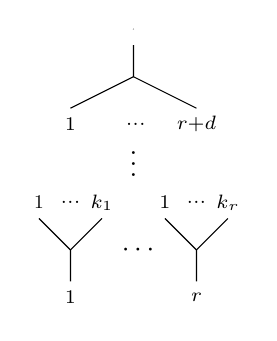
\begin{tikzpicture}[scale=.4]
	\node[scale=\r] at (5,8){\r};
	\draw (3,5.5)--(5,6.5)--(5,7.5);
	\draw (7,5.5)--(5,6.5);
	\node at (3,5){$\scriptstyle 1$};
	\node at (5,5){\,$\scriptstyle \dots$};
	\node at (7,5){$\scriptstyle r+d$};
	
	\node at (5,4){$\vdots$};
	
	\node at (3,-.5){$\scriptstyle 1$};
	\draw (2,2)--(3,1)--(3,0);
	\draw (4,2)--(3,1);
	\node[scale=.7] at (2,2.5){1};
	\node at (3,2.5){$\scriptstyle \dots$};
	\node at (4,2.5){$\scriptstyle k_1$};
	
	\node at (5,1){\ $\cdots$};
	
	\node at (7,-.5){$\scriptstyle r$};
	\draw (6,2)--(7,1)--(7,0);
	\draw (8,2)--(7,1);
	\node at (6,2.5){$\scriptstyle 1$};
	\node at (7,2.5){$\scriptstyle \dots$};
	\node at (8,2.5){$\scriptstyle k_r$};
	\end{tikzpicture}}
\end{center}
containing no internal vertices and such that for each $i = 1, \dots, r$ the induced map 
\begin{equation*}
\{1, \dots, k_i\} \to \{1, \dots, r+d\}
\end{equation*}
is order preserving.